% Options for packages loaded elsewhere
\PassOptionsToPackage{unicode}{hyperref}
\PassOptionsToPackage{hyphens}{url}
%
\documentclass[
]{article}
\usepackage{amsmath,amssymb}
\usepackage{iftex}
\ifPDFTeX
  \usepackage[T1]{fontenc}
  \usepackage[utf8]{inputenc}
  \usepackage{textcomp} % provide euro and other symbols
\else % if luatex or xetex
  \usepackage{unicode-math} % this also loads fontspec
  \defaultfontfeatures{Scale=MatchLowercase}
  \defaultfontfeatures[\rmfamily]{Ligatures=TeX,Scale=1}
\fi
\usepackage{lmodern}
\ifPDFTeX\else
  % xetex/luatex font selection
\fi
% Use upquote if available, for straight quotes in verbatim environments
\IfFileExists{upquote.sty}{\usepackage{upquote}}{}
\IfFileExists{microtype.sty}{% use microtype if available
  \usepackage[]{microtype}
  \UseMicrotypeSet[protrusion]{basicmath} % disable protrusion for tt fonts
}{}
\makeatletter
\@ifundefined{KOMAClassName}{% if non-KOMA class
  \IfFileExists{parskip.sty}{%
    \usepackage{parskip}
  }{% else
    \setlength{\parindent}{0pt}
    \setlength{\parskip}{6pt plus 2pt minus 1pt}}
}{% if KOMA class
  \KOMAoptions{parskip=half}}
\makeatother
\usepackage{xcolor}
\usepackage[margin=1in]{geometry}
\usepackage{color}
\usepackage{fancyvrb}
\newcommand{\VerbBar}{|}
\newcommand{\VERB}{\Verb[commandchars=\\\{\}]}
\DefineVerbatimEnvironment{Highlighting}{Verbatim}{commandchars=\\\{\}}
% Add ',fontsize=\small' for more characters per line
\usepackage{framed}
\definecolor{shadecolor}{RGB}{248,248,248}
\newenvironment{Shaded}{\begin{snugshade}}{\end{snugshade}}
\newcommand{\AlertTok}[1]{\textcolor[rgb]{0.94,0.16,0.16}{#1}}
\newcommand{\AnnotationTok}[1]{\textcolor[rgb]{0.56,0.35,0.01}{\textbf{\textit{#1}}}}
\newcommand{\AttributeTok}[1]{\textcolor[rgb]{0.13,0.29,0.53}{#1}}
\newcommand{\BaseNTok}[1]{\textcolor[rgb]{0.00,0.00,0.81}{#1}}
\newcommand{\BuiltInTok}[1]{#1}
\newcommand{\CharTok}[1]{\textcolor[rgb]{0.31,0.60,0.02}{#1}}
\newcommand{\CommentTok}[1]{\textcolor[rgb]{0.56,0.35,0.01}{\textit{#1}}}
\newcommand{\CommentVarTok}[1]{\textcolor[rgb]{0.56,0.35,0.01}{\textbf{\textit{#1}}}}
\newcommand{\ConstantTok}[1]{\textcolor[rgb]{0.56,0.35,0.01}{#1}}
\newcommand{\ControlFlowTok}[1]{\textcolor[rgb]{0.13,0.29,0.53}{\textbf{#1}}}
\newcommand{\DataTypeTok}[1]{\textcolor[rgb]{0.13,0.29,0.53}{#1}}
\newcommand{\DecValTok}[1]{\textcolor[rgb]{0.00,0.00,0.81}{#1}}
\newcommand{\DocumentationTok}[1]{\textcolor[rgb]{0.56,0.35,0.01}{\textbf{\textit{#1}}}}
\newcommand{\ErrorTok}[1]{\textcolor[rgb]{0.64,0.00,0.00}{\textbf{#1}}}
\newcommand{\ExtensionTok}[1]{#1}
\newcommand{\FloatTok}[1]{\textcolor[rgb]{0.00,0.00,0.81}{#1}}
\newcommand{\FunctionTok}[1]{\textcolor[rgb]{0.13,0.29,0.53}{\textbf{#1}}}
\newcommand{\ImportTok}[1]{#1}
\newcommand{\InformationTok}[1]{\textcolor[rgb]{0.56,0.35,0.01}{\textbf{\textit{#1}}}}
\newcommand{\KeywordTok}[1]{\textcolor[rgb]{0.13,0.29,0.53}{\textbf{#1}}}
\newcommand{\NormalTok}[1]{#1}
\newcommand{\OperatorTok}[1]{\textcolor[rgb]{0.81,0.36,0.00}{\textbf{#1}}}
\newcommand{\OtherTok}[1]{\textcolor[rgb]{0.56,0.35,0.01}{#1}}
\newcommand{\PreprocessorTok}[1]{\textcolor[rgb]{0.56,0.35,0.01}{\textit{#1}}}
\newcommand{\RegionMarkerTok}[1]{#1}
\newcommand{\SpecialCharTok}[1]{\textcolor[rgb]{0.81,0.36,0.00}{\textbf{#1}}}
\newcommand{\SpecialStringTok}[1]{\textcolor[rgb]{0.31,0.60,0.02}{#1}}
\newcommand{\StringTok}[1]{\textcolor[rgb]{0.31,0.60,0.02}{#1}}
\newcommand{\VariableTok}[1]{\textcolor[rgb]{0.00,0.00,0.00}{#1}}
\newcommand{\VerbatimStringTok}[1]{\textcolor[rgb]{0.31,0.60,0.02}{#1}}
\newcommand{\WarningTok}[1]{\textcolor[rgb]{0.56,0.35,0.01}{\textbf{\textit{#1}}}}
\usepackage{graphicx}
\makeatletter
\def\maxwidth{\ifdim\Gin@nat@width>\linewidth\linewidth\else\Gin@nat@width\fi}
\def\maxheight{\ifdim\Gin@nat@height>\textheight\textheight\else\Gin@nat@height\fi}
\makeatother
% Scale images if necessary, so that they will not overflow the page
% margins by default, and it is still possible to overwrite the defaults
% using explicit options in \includegraphics[width, height, ...]{}
\setkeys{Gin}{width=\maxwidth,height=\maxheight,keepaspectratio}
% Set default figure placement to htbp
\makeatletter
\def\fps@figure{htbp}
\makeatother
\setlength{\emergencystretch}{3em} % prevent overfull lines
\providecommand{\tightlist}{%
  \setlength{\itemsep}{0pt}\setlength{\parskip}{0pt}}
\setcounter{secnumdepth}{-\maxdimen} % remove section numbering
\usepackage{booktabs}
\usepackage{longtable}
\usepackage{array}
\usepackage{multirow}
\usepackage{wrapfig}
\usepackage{float}
\usepackage{colortbl}
\usepackage{pdflscape}
\usepackage{tabu}
\usepackage{threeparttable}
\usepackage{threeparttablex}
\usepackage[normalem]{ulem}
\usepackage{makecell}
\usepackage{xcolor}
\ifLuaTeX
  \usepackage{selnolig}  % disable illegal ligatures
\fi
\usepackage{bookmark}
\IfFileExists{xurl.sty}{\usepackage{xurl}}{} % add URL line breaks if available
\urlstyle{same}
\hypersetup{
  pdftitle={NYC Marathon},
  pdfauthor={Nicholas Jacob},
  hidelinks,
  pdfcreator={LaTeX via pandoc}}

\title{NYC Marathon}
\author{Nicholas Jacob}
\date{2025-04-08}

\begin{document}
\maketitle

\subsection{NYC Marathon 2024}\label{nyc-marathon-2024}

I really wanted to construct the project one more time during the
current semester for MATH 3583 Applied Stats. I figured I could express
some new coding techniques I have learned over the last four years and
hopefully get a little better at R.

For this project, I am using the NYC Marathon results from 2024. Here
are the first six finishers. Be careful about printing too much of the
data at any one time as it makes your report unreadable. I'll include
some of my code but often, I'll just make the outputs available when
appropriate.

\begin{Shaded}
\begin{Highlighting}[]
\NormalTok{df }\OtherTok{=} \FunctionTok{read.csv}\NormalTok{(}\StringTok{"NYCMarathon2024.csv"}\NormalTok{)}
\FunctionTok{head}\NormalTok{(df)}
\end{Highlighting}
\end{Shaded}

\begin{verbatim}
##   runnerId firstName bib age gender               city countryCode
## 1 41771195      Abdi   7  35      M           Nijmegen         NLD
## 2 41775746     Evans   3  35      M           Kapsabet         KEN
## 3 41766254    Albert   2  30      M          Kapkitony         KEN
## 4 41763160   Tamirat   1  33      M        Addis Ababa         ETH
## 5 41757406  Geoffrey   6  31      M Kapchorwa District         KEN
## 6 41772970    Conner  10  27      M              Provo         USA
##   stateProvince iaaf overallPlace overallTime pace genderPlace ageGradeTime
## 1                NED            1     2:07:39 4:53           1         6:57
## 2             -  KEN            2     2:07:45 4:53           2         7:03
## 3                KEN            3     2:08:00 4:53           3         8:00
## 4                ETH            4     2:08:12 4:54           4         8:02
## 5             -  KEN            5     2:08:50 4:55           5         8:50
## 6            UT  USA            6     2:09:00 4:56           6         9:00
##   ageGradePlace ageGradePercent racesCount
## 1             1           96.86          4
## 2             2           96.79          2
## 3             3           96.06          5
## 4             4           96.03          4
## 5             6           95.44          5
## 6             7           95.31          2
\end{verbatim}

I first want to give a little check on the quality of the data. I do
this with a large block of code that I have hidden away but show the
results only.

\begin{table}[H]
\centering
\caption{\label{tab:unnamed-chunk-6}Descriptive Summary of Numeric Variables}
\centering
\resizebox{\ifdim\width>\linewidth\linewidth\else\width\fi}{!}{
\fontsize{12}{14}\selectfont
\begin{tabular}[t]{lrrrrrrrrrrrr}
\toprule
\textbf{variable} & \textbf{n} & \textbf{missing} & \textbf{missing\_pct} & \textbf{unique} & \textbf{unique\_pct} & \textbf{mean} & \textbf{min} & \textbf{Q1} & \textbf{median} & \textbf{Q3} & \textbf{max} & \textbf{sd}\\
\midrule
runnerId & 55524 & 0 & 0.00 & 55524 & 100.00 & 4.2e+07 & 4.2e+07 & 4.2e+07 & 4.2e+07 & 4.2e+07 & 4.2e+07 & 16059\\
\addlinespace[0.5em]
bib & 55524 & 12 & 0.02 & 55513 & 99.98 & 3.3e+04 & 1.0e+00 & 1.7e+04 & 3.3e+04 & 4.9e+04 & 6.7e+04 & 18932\\
\addlinespace[0.5em]
age & 55524 & 0 & 0.00 & 70 & 0.13 & 4.0e+01 & 0.0e+00 & 3.0e+01 & 3.9e+01 & 4.8e+01 & 8.8e+01 & 12\\
\addlinespace[0.5em]
overallPlace & 55524 & 0 & 0.00 & 55524 & 100.00 & 2.8e+04 & 1.0e+00 & 1.4e+04 & 2.8e+04 & 4.2e+04 & 5.6e+04 & 16029\\
\addlinespace[0.5em]
genderPlace & 55524 & 0 & 0.00 & 30696 & 55.28 & 1.4e+04 & 1.0e+00 & 6.9e+03 & 1.4e+04 & 2.1e+04 & 3.1e+04 & 8287\\
\addlinespace[0.5em]
\addlinespace
ageGradePlace & 55524 & 0 & 0.00 & 30697 & 55.29 & 1.4e+04 & 0.0e+00 & 6.9e+03 & 1.4e+04 & 2.1e+04 & 3.1e+04 & 8287\\
\addlinespace[0.5em]
ageGradePercent & 55524 & 0 & 0.00 & 5603 & 10.09 & 5.2e+01 & 0.0e+00 & 4.5e+01 & 5.2e+01 & 5.9e+01 & 9.7e+01 & 11\\
\addlinespace[0.5em]
racesCount & 55524 & 0 & 0.00 & 315 & 0.57 & 1.3e+01 & 1.0e+00 & 1.0e+00 & 2.0e+00 & 1.2e+01 & 1.4e+03 & 30\\
\addlinespace[0.5em]
\bottomrule
\end{tabular}}
\end{table}

\begin{table}[H]
\centering
\caption{\label{tab:unnamed-chunk-9}Descriptive Summary of Categorical Variables}
\centering
\fontsize{7}{9}\selectfont
\begin{tabular}[t]{lllrlrllll}
\toprule
\textbf{variable} & \textbf{n} & \textbf{missing} & \textbf{miss\_pct} & \textbf{unique} & \textbf{unique\_pct} & \textbf{mode} & \textbf{mode\_freq} & \textbf{least common} & \textbf{freq}\\
\midrule
firstName & 55524 & 0 & 0.00 & 12463 & 22.45 & Michael & 595 & A. AlLEXANDER & 1\\
\addlinespace[0.25em]\\
gender & 55524 & 0 & 0.00 & 4 & 0.01 & M & 30692 &  & 12\\
\addlinespace[0.25em]\\
city & 55524 & 0 & 0.00 & 10604 & 19.10 & New York & 10355 & (Select Country) & 1\\
\addlinespace[0.25em]
countryCode & 55524 & 0 & 0.00 & 137 & 0.25 & USA & 37695 & ABW & 1\\
\addlinespace[0.25em]\\
stateProvince & 55524 & 13 & 0.02 & 2351 & 4.23 & NY & 21372 & --- Please Select --- & 1\\
\addlinespace[0.25em]\\
\addlinespace
iaaf & 55524 & 1 & 0.00 & 161 & 0.29 & USA & 33361 & AHO & 1\\
\addlinespace[0.25em]\\
overallTime & 55524 & 0 & 0.00 & 14838 & 26.72 & 3:42:24 & 17 & 10:00:53 & 1\\
\addlinespace[0.25em]\\
pace & 55524 & 0 & 0.00 & 966 & 1.74 & 9:05 & 230 & 17:46 & 1\\
\addlinespace[0.25em]\\
ageGradeTime & 55524 & 0 & 0.00 & 3600 & 6.48 & 0:00 & 132 & 30:01:00 & 3\\
\addlinespace[0.25em]\\
\bottomrule
\end{tabular}
\end{table}

If you go back and look at the code, you'll see that is a lot of work to
make this pretty table. You are welcome to use this code but with so
much going on, it is difficult to debug\ldots{}

There are a couple of issues I am noticing in the current code. First
off, \texttt{countryCode} and \texttt{iaaf} look very similar but the
summary statistics are different so not sure what is going on with that.
Not a huge issue. The big issue I see is that the \texttt{overallTime}
is being interpreted as a categorical field. This will need to be fixed!

\subsection{Data Cleaning}\label{data-cleaning}

I like to do my data cleaning in the programming language I am using. It
will make it so that you don't need to touch or change the data at all
and you should be able to recreate what you did right after you load the
data. This way it will work for all other parts of the project.

Let's talk for a moment about my process for solving this problem. I
think I have done this before but I don't remember exactly how to do it.
First I take a guess at what this would be called. I know it isn't a
time but a time difference, so I search google with ``r time
difference''. At first I get a bit distracted by the first entry but
eventually I see the ETH Zurich site. This one is the R manual. There I
see that there is a data class called \texttt{difftime}. I skim the top
parts and go to the example which seems to do what I want. You see below
that it prints the winners time in hours as I had hoped!

\begin{Shaded}
\begin{Highlighting}[]
\FunctionTok{as.difftime}\NormalTok{(df}\SpecialCharTok{$}\NormalTok{overallTime)[}\DecValTok{1}\NormalTok{]}
\end{Highlighting}
\end{Shaded}

\begin{verbatim}
## Time difference of 2.13 hours
\end{verbatim}

I can also convert that the seconds if I wanted to. The \texttt{{[}1{]}}
is limiting the printout just to the very first entry.

\begin{Shaded}
\begin{Highlighting}[]
\FunctionTok{as.difftime}\NormalTok{(df}\SpecialCharTok{$}\NormalTok{overallTime, }\AttributeTok{units =} \StringTok{"secs"}\NormalTok{)[}\DecValTok{1}\NormalTok{]}
\end{Highlighting}
\end{Shaded}

\begin{verbatim}
## Time difference of 7659 secs
\end{verbatim}

So I will mutate the time columns so that we can continue our analysis.

\begin{Shaded}
\begin{Highlighting}[]
\NormalTok{df }\OtherTok{\textless{}{-}}\NormalTok{ df }\SpecialCharTok{\%\textgreater{}\%} \FunctionTok{mutate}\NormalTok{(}
  \AttributeTok{overallTime =} \FunctionTok{as.difftime}\NormalTok{(overallTime)}
\NormalTok{)}
\end{Highlighting}
\end{Shaded}

Dang it! That worked for te overall time but not for \texttt{pace} nor
\texttt{ageGradeTime}. Since I am not sure what \texttt{ageGradeTime}
is, I'll just not use it in any analysis. I'll recompute pace by taking
the \texttt{overallTime} and dividing by the length of the Marathon
(26.2 miles) Notice how content knowledge is important to dealing with
your data?

\begin{Shaded}
\begin{Highlighting}[]
\NormalTok{df }\OtherTok{\textless{}{-}}\NormalTok{ df }\SpecialCharTok{\%\textgreater{}\%} \FunctionTok{mutate}\NormalTok{(}
  \AttributeTok{pace =} \FunctionTok{ms}\NormalTok{(pace), }\CommentTok{\#using lubridate and convert og pace}
  \AttributeTok{pace2 =}\NormalTok{ overallTime}\SpecialCharTok{/}\FloatTok{26.2} \CommentTok{\# just divide by length.  Gives pace in hours}
\NormalTok{)}
\end{Highlighting}
\end{Shaded}

\begin{verbatim}
## Warning: There was 1 warning in `mutate()`.
## i In argument: `pace = ms(pace)`.
## Caused by warning in `.parse_hms()`:
## ! Some strings failed to parse
\end{verbatim}

Well, I could get the division to work but I couldn't seem to get it in
an hour format. I left it here as called \texttt{pace2}. I did find the
tidy version for dealing with dates and times called \texttt{lubridate}.
This is a library I had to add to the beginning of my document. Now,
\texttt{pace} has minutes and seconds.

Okay so your data will have some cleaning that is needed. You'll need to
start early! Cleaning is a pain and you may need some of my help to get
it in a good format. Once the data is clean, you shouldn't need to do
that again!

\subsection{Exploratory Data Analysis}\label{exploratory-data-analysis}

While I already did some of the EDA in my data summary table, I should
show some easier to understand code for this too. Here is summary of the
times.

\begin{Shaded}
\begin{Highlighting}[]
\FunctionTok{summary}\NormalTok{(}\FunctionTok{as.numeric}\NormalTok{(df}\SpecialCharTok{$}\NormalTok{overallTime))}
\end{Highlighting}
\end{Shaded}

\begin{verbatim}
##    Min. 1st Qu.  Median    Mean 3rd Qu.    Max. 
##    2.13    3.81    4.39    4.53    5.09   11.80
\end{verbatim}

I am missing standard deviation, so I add that inline showing that the
standard deviation, 1.03. Here is used the code \texttt{sd} and if there
had been na values, I would have added the option
\texttt{na.rm\ =\ TRUE}.

I add the graphical displays using the \texttt{ggplot2} package (I am a
big fan!) You can do these in base r but I'll stick to ggplot as it has
so many options to make beautiful graphics.

\begin{Shaded}
\begin{Highlighting}[]
\FunctionTok{ggplot}\NormalTok{(}\AttributeTok{data =}\NormalTok{ df, }\FunctionTok{aes}\NormalTok{(}\AttributeTok{x =} \FunctionTok{as.numeric}\NormalTok{(overallTime)))}\SpecialCharTok{+}
  \FunctionTok{geom\_histogram}\NormalTok{()}
\end{Highlighting}
\end{Shaded}

\begin{verbatim}
## `stat_bin()` using `bins = 30`. Pick better value with `binwidth`.
\end{verbatim}

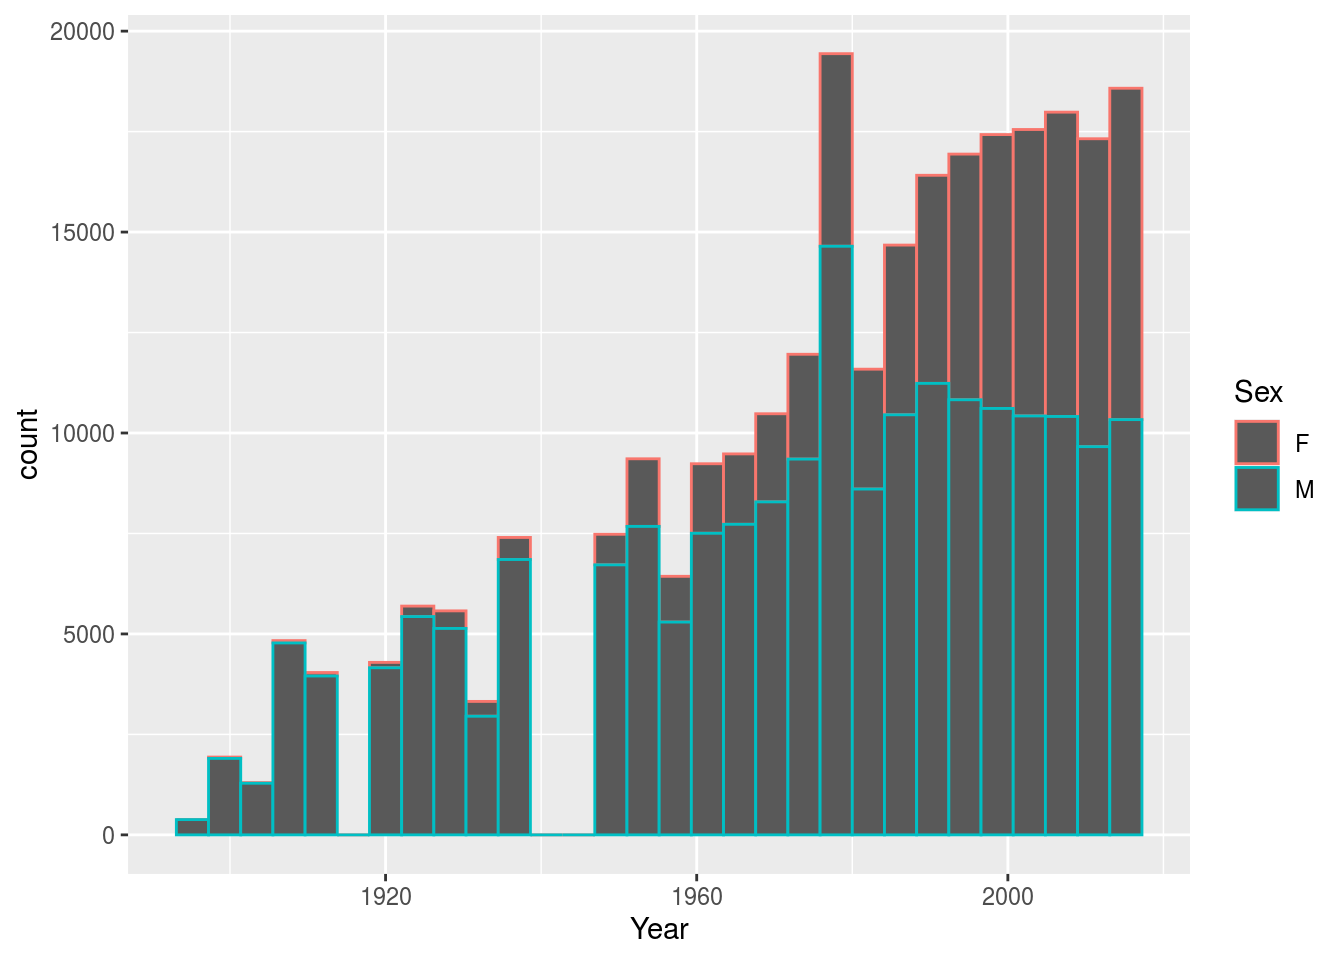
\includegraphics{NYCMarathonProject_files/figure-latex/unnamed-chunk-15-1.pdf}

\begin{Shaded}
\begin{Highlighting}[]
\FunctionTok{ggplot}\NormalTok{(}\AttributeTok{data =}\NormalTok{ df, }\FunctionTok{aes}\NormalTok{(}\AttributeTok{x =} \FunctionTok{as.numeric}\NormalTok{(overallTime)))}\SpecialCharTok{+}
  \FunctionTok{geom\_boxplot}\NormalTok{() }\SpecialCharTok{+}
  \FunctionTok{labs}\NormalTok{(}\AttributeTok{x =} \StringTok{"Time in hours"}\NormalTok{,}
       \AttributeTok{title =} \StringTok{"Boxplot of runners time in NYC Marathon"}\NormalTok{)}\SpecialCharTok{+}
  \FunctionTok{theme}\NormalTok{(}\AttributeTok{axis.text.y=}\FunctionTok{element\_blank}\NormalTok{(),}\AttributeTok{axis.ticks.y=}\FunctionTok{element\_blank}\NormalTok{())}
\end{Highlighting}
\end{Shaded}

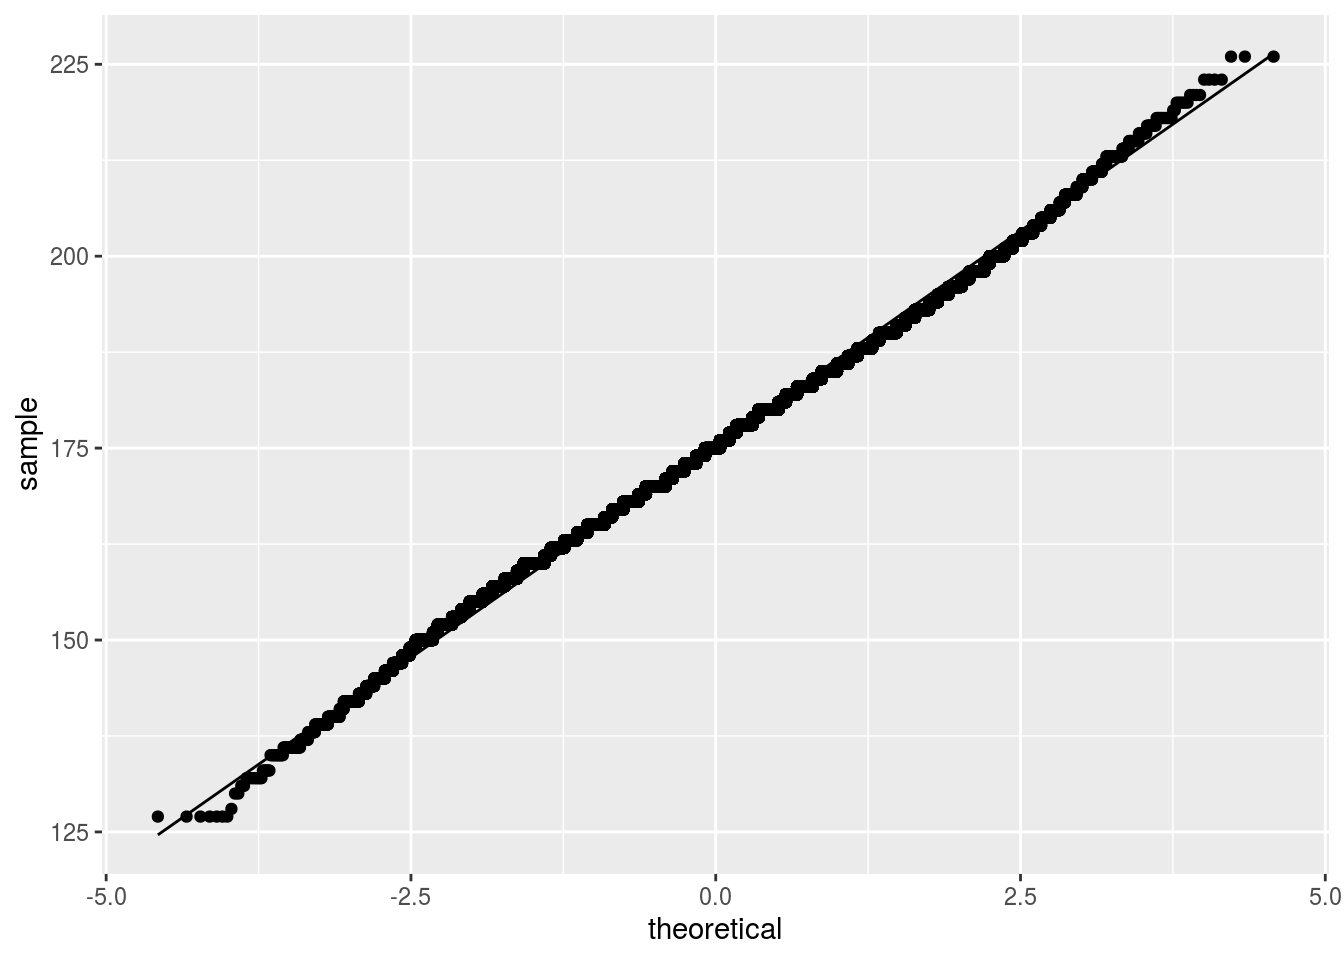
\includegraphics{NYCMarathonProject_files/figure-latex/unnamed-chunk-16-1.pdf}
We do see the outliers on the boxplot. These are categorized as values
that are more (or less) than \(1.5IQR\) beyond the \(Q_3\) (or \(Q_1\)
for below). Let's do a proper statistical test looking for outliers.

\begin{Shaded}
\begin{Highlighting}[]
\FunctionTok{grubbs.test}\NormalTok{(}\FunctionTok{as.numeric}\NormalTok{(df}\SpecialCharTok{$}\NormalTok{overallTime))}
\end{Highlighting}
\end{Shaded}

\begin{verbatim}
## 
##  Grubbs test for one outlier
## 
## data:  as.numeric(df$overallTime)
## G = 7, U = 1, p-value = 0.00000005
## alternative hypothesis: highest value 11.7986111111111 is an outlier
\end{verbatim}

So the highest value is clearly an outlier. Of course the issue here is
that this test only looks at that one outlier.

For the categorical variable, we can do some similarly straight forward
coding

\begin{Shaded}
\begin{Highlighting}[]
\FunctionTok{table}\NormalTok{(df}\SpecialCharTok{$}\NormalTok{countryCode)[}\DecValTok{1}\SpecialCharTok{:}\DecValTok{10}\NormalTok{]}\CommentTok{\#this limited me to 10 entries}
\end{Highlighting}
\end{Shaded}

\begin{verbatim}
## 
##     ABW AGO AND ANT ARE ARG ARM AUS AUT 
##  12   1   1   3  59  51 185   1 710 107
\end{verbatim}

12 blanks is a little odd. I can do this another way that may give you a
better look.

\begin{Shaded}
\begin{Highlighting}[]
\NormalTok{df }\SpecialCharTok{\%\textgreater{}\%} \FunctionTok{group\_by}\NormalTok{(countryCode)}\SpecialCharTok{\%\textgreater{}\%}
  \FunctionTok{summarise}\NormalTok{(}\AttributeTok{count =} \FunctionTok{n}\NormalTok{()) }\SpecialCharTok{\%\textgreater{}\%}
  \FunctionTok{mutate}\NormalTok{( }\AttributeTok{freq\_pct =}\NormalTok{ count}\SpecialCharTok{/}\FunctionTok{length}\NormalTok{(df}\SpecialCharTok{$}\NormalTok{runnerId)}\SpecialCharTok{*}\DecValTok{100}\NormalTok{) }\SpecialCharTok{\%\textgreater{}\%}
  \FunctionTok{head}\NormalTok{()}
\end{Highlighting}
\end{Shaded}

\begin{verbatim}
## # A tibble: 6 x 3
##   countryCode count freq_pct
##   <chr>       <int>    <dbl>
## 1 ""             12  0.0216 
## 2 "ABW"           1  0.00180
## 3 "AGO"           1  0.00180
## 4 "AND"           3  0.00540
## 5 "ANT"          59  0.106  
## 6 "ARE"          51  0.0919
\end{verbatim}

For the two-way table, I'll repeat with two methods. Here is the base
method, again restricting so I don't show too much

\begin{Shaded}
\begin{Highlighting}[]
\FunctionTok{table}\NormalTok{(df}\SpecialCharTok{$}\NormalTok{countryCode,df}\SpecialCharTok{$}\NormalTok{iaaf)[}\DecValTok{1}\SpecialCharTok{:}\DecValTok{10}\NormalTok{,}\DecValTok{1}\SpecialCharTok{:}\DecValTok{10}\NormalTok{]}
\end{Highlighting}
\end{Shaded}

\begin{verbatim}
##      
##           AFG AHO ALB ALG AND ANG ANT ARG ARM
##        12   0   0   0   0   0   0   0   0   0
##   ABW   0   0   0   0   0   0   0   0   0   0
##   AGO   0   0   0   0   0   0   1   0   0   0
##   AND   0   0   0   0   0   0   0   0   0   0
##   ANT   0   0   1   0   0   0   0   1   0   0
##   ARE   0   0   0   0   0   0   0   0   0   0
##   ARG   0   0   0   0   0   0   0   0 174   0
##   ARM   0   0   0   0   0   0   0   0   0   1
##   AUS   0   0   0   0   0   0   0   0   0   0
##   AUT   0   0   0   0   0   0   0   0   0   0
\end{verbatim}

As for the tidy version:

\begin{Shaded}
\begin{Highlighting}[]
\NormalTok{df }\SpecialCharTok{\%\textgreater{}\%} \FunctionTok{count}\NormalTok{(countryCode,iaaf)}\SpecialCharTok{\%\textgreater{}\%}
  \FunctionTok{head}\NormalTok{()}
\end{Highlighting}
\end{Shaded}

\begin{verbatim}
##   countryCode iaaf  n
## 1                  12
## 2         ABW  ARU  1
## 3         AGO  ANG  1
## 4         AND  AUS  1
## 5         AND  ESP  1
## 6         AND  GBR  1
\end{verbatim}

This doesn't look like a two-way but it has the same data. (I couldn't
find the method to change it to a table quickly so I am happy as is.)

\subsection{Hypothesis Testing}\label{hypothesis-testing}

You can get pretty crazy with your hypotheses. I just ask that you
explore something of interest based on your content knowledge. For me, I
am interested in playing around with names. I am going to test if people
named Nicholas have a different average time in the race from those
named Micheal (our mode). I'll state this formally as \[
H_0:\quad \mu_{Nicholas} = \mu_{Micheal}
\] \[
H_a:\quad \mu_{Nicholas} \neq \mu_{Micheal}
\]

To continue, I'll need to subset my data. This is actually not too hard
but has some quirks. Using the \$ to get to the variable in the dataset,
I ask it be logically equal to what I am looking for.

\begin{Shaded}
\begin{Highlighting}[]
\FunctionTok{head}\NormalTok{(df}\SpecialCharTok{$}\NormalTok{firstName }\SpecialCharTok{==} \StringTok{"Nicholas"}\NormalTok{)}
\end{Highlighting}
\end{Shaded}

\begin{verbatim}
## [1] FALSE FALSE FALSE FALSE FALSE FALSE
\end{verbatim}

This gives a bunch of True/False. To get the data from that, we pass it
into the dataframe

\begin{Shaded}
\begin{Highlighting}[]
\FunctionTok{head}\NormalTok{(df[df}\SpecialCharTok{$}\NormalTok{firstName }\SpecialCharTok{==} \StringTok{"Nicholas"}\NormalTok{,]) }\CommentTok{\#163 is still too many to print them all!}
\end{Highlighting}
\end{Shaded}

\begin{verbatim}
##     runnerId firstName  bib age gender           city countryCode stateProvince
## 241 41788330  Nicholas 1364  24      M           Reno         USA            NV
## 382 41780288  Nicholas  604  24      M        Memphis         USA            TN
## 404 41772035  Nicholas  693  28      M       New York         USA            NY
## 534 41790532  Nicholas 1866  29      M Salt Lake City         USA            UT
## 541 41758256  Nicholas  773  34      M       New York         USA            NY
## 662 41764548  Nicholas 4526  29      M     Park Ridge         USA            IL
##     iaaf overallPlace overallTime   pace genderPlace ageGradeTime ageGradePlace
## 241  USA          241  2.58 hours 5M 55S         220     35:05:00           472
## 382  USA          382  2.66 hours  6M 5S         354     39:27:00           794
## 404  USA          404  2.67 hours  6M 7S         376     40:04:00           846
## 534  USA          534  2.72 hours 6M 13S         498     42:55:00          1075
## 541  USA          541  2.72 hours 6M 14S         505     42:35:00          1049
## 662  USA          662  2.75 hours 6M 18S         616     44:56:00          1271
##     ageGradePercent racesCount        pace2
## 241            79.3          1 0.0987 hours
## 382            77.1          1 0.1014 hours
## 404            76.8         19 0.1018 hours
## 534            75.5          1 0.1036 hours
## 541            75.6         37 0.1037 hours
## 662            74.5          6 0.1049 hours
\end{verbatim}

Lastly, I get the data I want by taking the subsetted data and asking
for that variable with the \$ sign again. Now I want the
\texttt{overallTime}. I've dropped this into my \texttt{t.test} to
preform the test.

\begin{Shaded}
\begin{Highlighting}[]
\NormalTok{ttest }\OtherTok{\textless{}{-}}\FunctionTok{t.test}\NormalTok{(}\FunctionTok{as.numeric}\NormalTok{(df[df}\SpecialCharTok{$}\NormalTok{firstName }\SpecialCharTok{==} \StringTok{"Nicholas"}\NormalTok{,]}\SpecialCharTok{$}\NormalTok{overallTime),}
        \FunctionTok{as.numeric}\NormalTok{(df[df}\SpecialCharTok{$}\NormalTok{firstName }\SpecialCharTok{==} \StringTok{"Michael"}\NormalTok{,]}\SpecialCharTok{$}\NormalTok{overallTime))}

\NormalTok{ttest}
\end{Highlighting}
\end{Shaded}

\begin{verbatim}
## 
##  Welch Two Sample t-test
## 
## data:  as.numeric(df[df$firstName == "Nicholas", ]$overallTime) and as.numeric(df[df$firstName == "Michael", ]$overallTime)
## t = -4, df = 322, p-value = 0.00007
## alternative hypothesis: true difference in means is not equal to 0
## 95 percent confidence interval:
##  -0.474 -0.164
## sample estimates:
## mean of x mean of y 
##      4.05      4.37
\end{verbatim}

The results above are printed but we can access the data in other ways
too. We can say that this test gave us a \(p\)-value of 0.

So we see these are different but we should look at some visualizations
to confirm.
\includegraphics{NYCMarathonProject_files/figure-latex/unnamed-chunk-25-1.pdf}

\subsection{Goodness of Fit}\label{goodness-of-fit}

\subsubsection{Test for Idependence}\label{test-for-idependence}

We expect all people from USA also have a country code for the US. Let's
test this.

\begin{Shaded}
\begin{Highlighting}[]
\NormalTok{test }\OtherTok{\textless{}{-}} \FunctionTok{chisq.test}\NormalTok{(}\FunctionTok{table}\NormalTok{(df[df}\SpecialCharTok{$}\NormalTok{iaaf }\SpecialCharTok{==} \StringTok{"USA"}\NormalTok{,}\StringTok{"countryCode"}\NormalTok{]))}
\NormalTok{test}
\end{Highlighting}
\end{Shaded}

\begin{verbatim}
## 
##  Chi-squared test for given probabilities
## 
## data:  table(df[df$iaaf == "USA", "countryCode"])
## X-squared = 1416456, df = 43, p-value <0.0000000000000002
\end{verbatim}

So this was the expected table. What did the actual table look like?

\begin{Shaded}
\begin{Highlighting}[]
\NormalTok{test}\SpecialCharTok{$}\NormalTok{expected}
\end{Highlighting}
\end{Shaded}

\begin{verbatim}
## ARE ARG AUS BEL BRA BRB CAN CHE CHI CHL CHN COL DEU DOM ECU EGY ESP FRA GBR GIB 
## 758 758 758 758 758 758 758 758 758 758 758 758 758 758 758 758 758 758 758 758 
## GRC HKG HND IDN IND IRL ISR ITA JAM JPN KOR MAR MEX NLD NOR NZL POL PRI SGP SLV 
## 758 758 758 758 758 758 758 758 758 758 758 758 758 758 758 758 758 758 758 758 
## THA USA VEN ZAF 
## 758 758 758 758
\end{verbatim}

\begin{Shaded}
\begin{Highlighting}[]
\FunctionTok{table}\NormalTok{(df[df}\SpecialCharTok{$}\NormalTok{iaaf }\SpecialCharTok{==} \StringTok{"USA"}\NormalTok{,}\StringTok{"countryCode"}\NormalTok{])}
\end{Highlighting}
\end{Shaded}

\begin{verbatim}
## 
##   ARE   ARG   AUS   BEL   BRA   BRB   CAN   CHE   CHI   CHL   CHN   COL   DEU 
##     3     3     4     2     3     1    13     5     1     1     5     4     6 
##   DOM   ECU   EGY   ESP   FRA   GBR   GIB   GRC   HKG   HND   IDN   IND   IRL 
##     1     2     2     2     7    43     1     1     4     2     1     8     4 
##   ISR   ITA   JAM   JPN   KOR   MAR   MEX   NLD   NOR   NZL   POL   PRI   SGP 
##     9     7     1     2     7     1    31     7     1     2     1     1     2 
##   SLV   THA   USA   VEN   ZAF 
##     2     1 33155     1     1
\end{verbatim}

Yes, most were from the US.

\subsubsection{Contingency Table}\label{contingency-table}

Now I need a two way table. I don't print it because it is annoyingly
large.

\begin{Shaded}
\begin{Highlighting}[]
\FunctionTok{chisq.test}\NormalTok{(}\FunctionTok{table}\NormalTok{(df[df}\SpecialCharTok{$}\NormalTok{iaaf }\SpecialCharTok{==} \StringTok{"USA"}\NormalTok{,}\StringTok{"countryCode"}\NormalTok{],df[df}\SpecialCharTok{$}\NormalTok{iaaf }\SpecialCharTok{==} \StringTok{"USA"}\NormalTok{,}\StringTok{"stateProvince"}\NormalTok{]))}
\end{Highlighting}
\end{Shaded}

\begin{verbatim}
## Warning in chisq.test(table(df[df$iaaf == "USA", "countryCode"], df[df$iaaf ==
## : Chi-squared approximation may be incorrect
\end{verbatim}

\begin{verbatim}
## 
##  Pearson's Chi-squared test
## 
## data:  table(df[df$iaaf == "USA", "countryCode"], df[df$iaaf == "USA",     "stateProvince"])
## X-squared = 1320775, df = 9374, p-value <0.0000000000000002
\end{verbatim}

\begin{Shaded}
\begin{Highlighting}[]
\FunctionTok{mosaicplot}\NormalTok{(}\FunctionTok{table}\NormalTok{(df[df}\SpecialCharTok{$}\NormalTok{iaaf }\SpecialCharTok{==} \StringTok{"USA"}\NormalTok{,}\StringTok{"countryCode"}\NormalTok{],df[df}\SpecialCharTok{$}\NormalTok{iaaf }\SpecialCharTok{==} \StringTok{"USA"}\NormalTok{,}\StringTok{"stateProvince"}\NormalTok{]))}
\end{Highlighting}
\end{Shaded}

\begin{verbatim}
## Warning in text.default(x = 35 * cex.axis/0.66 - 20 * cex.axis/0.66 * (lablevy
## - : conversion failure on 'ニューヨーク州' in 'mbcsToSbcs': dot substituted for
## <e3>
\end{verbatim}

\begin{verbatim}
## Warning in text.default(x = 35 * cex.axis/0.66 - 20 * cex.axis/0.66 * (lablevy
## - : conversion failure on 'ニューヨーク州' in 'mbcsToSbcs': dot substituted for
## <83>
\end{verbatim}

\begin{verbatim}
## Warning in text.default(x = 35 * cex.axis/0.66 - 20 * cex.axis/0.66 * (lablevy
## - : conversion failure on 'ニューヨーク州' in 'mbcsToSbcs': dot substituted for
## <8b>
\end{verbatim}

\begin{verbatim}
## Warning in text.default(x = 35 * cex.axis/0.66 - 20 * cex.axis/0.66 * (lablevy
## - : conversion failure on 'ニューヨーク州' in 'mbcsToSbcs': dot substituted for
## <e3>
\end{verbatim}

\begin{verbatim}
## Warning in text.default(x = 35 * cex.axis/0.66 - 20 * cex.axis/0.66 * (lablevy
## - : conversion failure on 'ニューヨーク州' in 'mbcsToSbcs': dot substituted for
## <83>
\end{verbatim}

\begin{verbatim}
## Warning in text.default(x = 35 * cex.axis/0.66 - 20 * cex.axis/0.66 * (lablevy
## - : conversion failure on 'ニューヨーク州' in 'mbcsToSbcs': dot substituted for
## <a5>
\end{verbatim}

\begin{verbatim}
## Warning in text.default(x = 35 * cex.axis/0.66 - 20 * cex.axis/0.66 * (lablevy
## - : conversion failure on 'ニューヨーク州' in 'mbcsToSbcs': dot substituted for
## <e3>
\end{verbatim}

\begin{verbatim}
## Warning in text.default(x = 35 * cex.axis/0.66 - 20 * cex.axis/0.66 * (lablevy
## - : conversion failure on 'ニューヨーク州' in 'mbcsToSbcs': dot substituted for
## <83>
\end{verbatim}

\begin{verbatim}
## Warning in text.default(x = 35 * cex.axis/0.66 - 20 * cex.axis/0.66 * (lablevy
## - : conversion failure on 'ニューヨーク州' in 'mbcsToSbcs': dot substituted for
## <bc>
\end{verbatim}

\begin{verbatim}
## Warning in text.default(x = 35 * cex.axis/0.66 - 20 * cex.axis/0.66 * (lablevy
## - : conversion failure on 'ニューヨーク州' in 'mbcsToSbcs': dot substituted for
## <e3>
\end{verbatim}

\begin{verbatim}
## Warning in text.default(x = 35 * cex.axis/0.66 - 20 * cex.axis/0.66 * (lablevy
## - : conversion failure on 'ニューヨーク州' in 'mbcsToSbcs': dot substituted for
## <83>
\end{verbatim}

\begin{verbatim}
## Warning in text.default(x = 35 * cex.axis/0.66 - 20 * cex.axis/0.66 * (lablevy
## - : conversion failure on 'ニューヨーク州' in 'mbcsToSbcs': dot substituted for
## <a8>
\end{verbatim}

\begin{verbatim}
## Warning in text.default(x = 35 * cex.axis/0.66 - 20 * cex.axis/0.66 * (lablevy
## - : conversion failure on 'ニューヨーク州' in 'mbcsToSbcs': dot substituted for
## <e3>
\end{verbatim}

\begin{verbatim}
## Warning in text.default(x = 35 * cex.axis/0.66 - 20 * cex.axis/0.66 * (lablevy
## - : conversion failure on 'ニューヨーク州' in 'mbcsToSbcs': dot substituted for
## <83>
\end{verbatim}

\begin{verbatim}
## Warning in text.default(x = 35 * cex.axis/0.66 - 20 * cex.axis/0.66 * (lablevy
## - : conversion failure on 'ニューヨーク州' in 'mbcsToSbcs': dot substituted for
## <bc>
\end{verbatim}

\begin{verbatim}
## Warning in text.default(x = 35 * cex.axis/0.66 - 20 * cex.axis/0.66 * (lablevy
## - : conversion failure on 'ニューヨーク州' in 'mbcsToSbcs': dot substituted for
## <e3>
\end{verbatim}

\begin{verbatim}
## Warning in text.default(x = 35 * cex.axis/0.66 - 20 * cex.axis/0.66 * (lablevy
## - : conversion failure on 'ニューヨーク州' in 'mbcsToSbcs': dot substituted for
## <82>
\end{verbatim}

\begin{verbatim}
## Warning in text.default(x = 35 * cex.axis/0.66 - 20 * cex.axis/0.66 * (lablevy
## - : conversion failure on 'ニューヨーク州' in 'mbcsToSbcs': dot substituted for
## <af>
\end{verbatim}

\begin{verbatim}
## Warning in text.default(x = 35 * cex.axis/0.66 - 20 * cex.axis/0.66 * (lablevy
## - : conversion failure on 'ニューヨーク州' in 'mbcsToSbcs': dot substituted for
## <e5>
\end{verbatim}

\begin{verbatim}
## Warning in text.default(x = 35 * cex.axis/0.66 - 20 * cex.axis/0.66 * (lablevy
## - : conversion failure on 'ニューヨーク州' in 'mbcsToSbcs': dot substituted for
## <b7>
\end{verbatim}

\begin{verbatim}
## Warning in text.default(x = 35 * cex.axis/0.66 - 20 * cex.axis/0.66 * (lablevy
## - : conversion failure on 'ニューヨーク州' in 'mbcsToSbcs': dot substituted for
## <9e>
\end{verbatim}

\begin{verbatim}
## Warning in text.default(x = 35 * cex.axis/0.66 - 20 * cex.axis/0.66 * (lablevy
## - : font metrics unknown for Unicode character U+30CB
\end{verbatim}

\begin{verbatim}
## Warning in text.default(x = 35 * cex.axis/0.66 - 20 * cex.axis/0.66 * (lablevy
## - : font metrics unknown for Unicode character U+30E5
\end{verbatim}

\begin{verbatim}
## Warning in text.default(x = 35 * cex.axis/0.66 - 20 * cex.axis/0.66 * (lablevy
## - : font metrics unknown for Unicode character U+30FC
\end{verbatim}

\begin{verbatim}
## Warning in text.default(x = 35 * cex.axis/0.66 - 20 * cex.axis/0.66 * (lablevy
## - : font metrics unknown for Unicode character U+30E8
\end{verbatim}

\begin{verbatim}
## Warning in text.default(x = 35 * cex.axis/0.66 - 20 * cex.axis/0.66 * (lablevy
## - : font metrics unknown for Unicode character U+30FC
\end{verbatim}

\begin{verbatim}
## Warning in text.default(x = 35 * cex.axis/0.66 - 20 * cex.axis/0.66 * (lablevy
## - : font metrics unknown for Unicode character U+30AF
\end{verbatim}

\begin{verbatim}
## Warning in text.default(x = 35 * cex.axis/0.66 - 20 * cex.axis/0.66 * (lablevy
## - : font metrics unknown for Unicode character U+5DDE
\end{verbatim}

\begin{verbatim}
## Warning in text.default(x = 35 * cex.axis/0.66 - 20 * cex.axis/0.66 * (lablevy
## - : conversion failure on '경상북도' in 'mbcsToSbcs': dot substituted for <ea>
\end{verbatim}

\begin{verbatim}
## Warning in text.default(x = 35 * cex.axis/0.66 - 20 * cex.axis/0.66 * (lablevy
## - : conversion failure on '경상북도' in 'mbcsToSbcs': dot substituted for <b2>
\end{verbatim}

\begin{verbatim}
## Warning in text.default(x = 35 * cex.axis/0.66 - 20 * cex.axis/0.66 * (lablevy
## - : conversion failure on '경상북도' in 'mbcsToSbcs': dot substituted for <bd>
\end{verbatim}

\begin{verbatim}
## Warning in text.default(x = 35 * cex.axis/0.66 - 20 * cex.axis/0.66 * (lablevy
## - : conversion failure on '경상북도' in 'mbcsToSbcs': dot substituted for <ec>
\end{verbatim}

\begin{verbatim}
## Warning in text.default(x = 35 * cex.axis/0.66 - 20 * cex.axis/0.66 * (lablevy
## - : conversion failure on '경상북도' in 'mbcsToSbcs': dot substituted for <83>
\end{verbatim}

\begin{verbatim}
## Warning in text.default(x = 35 * cex.axis/0.66 - 20 * cex.axis/0.66 * (lablevy
## - : conversion failure on '경상북도' in 'mbcsToSbcs': dot substituted for <81>
\end{verbatim}

\begin{verbatim}
## Warning in text.default(x = 35 * cex.axis/0.66 - 20 * cex.axis/0.66 * (lablevy
## - : conversion failure on '경상북도' in 'mbcsToSbcs': dot substituted for <eb>
\end{verbatim}

\begin{verbatim}
## Warning in text.default(x = 35 * cex.axis/0.66 - 20 * cex.axis/0.66 * (lablevy
## - : conversion failure on '경상북도' in 'mbcsToSbcs': dot substituted for <b6>
\end{verbatim}

\begin{verbatim}
## Warning in text.default(x = 35 * cex.axis/0.66 - 20 * cex.axis/0.66 * (lablevy
## - : conversion failure on '경상북도' in 'mbcsToSbcs': dot substituted for <81>
\end{verbatim}

\begin{verbatim}
## Warning in text.default(x = 35 * cex.axis/0.66 - 20 * cex.axis/0.66 * (lablevy
## - : conversion failure on '경상북도' in 'mbcsToSbcs': dot substituted for <eb>
\end{verbatim}

\begin{verbatim}
## Warning in text.default(x = 35 * cex.axis/0.66 - 20 * cex.axis/0.66 * (lablevy
## - : conversion failure on '경상북도' in 'mbcsToSbcs': dot substituted for <8f>
\end{verbatim}

\begin{verbatim}
## Warning in text.default(x = 35 * cex.axis/0.66 - 20 * cex.axis/0.66 * (lablevy
## - : conversion failure on '경상북도' in 'mbcsToSbcs': dot substituted for <84>
\end{verbatim}

\begin{verbatim}
## Warning in text.default(x = 35 * cex.axis/0.66 - 20 * cex.axis/0.66 * (lablevy
## - : font metrics unknown for Unicode character U+ACBD
\end{verbatim}

\begin{verbatim}
## Warning in text.default(x = 35 * cex.axis/0.66 - 20 * cex.axis/0.66 * (lablevy
## - : font metrics unknown for Unicode character U+C0C1
\end{verbatim}

\begin{verbatim}
## Warning in text.default(x = 35 * cex.axis/0.66 - 20 * cex.axis/0.66 * (lablevy
## - : font metrics unknown for Unicode character U+BD81
\end{verbatim}

\begin{verbatim}
## Warning in text.default(x = 35 * cex.axis/0.66 - 20 * cex.axis/0.66 * (lablevy
## - : font metrics unknown for Unicode character U+B3C4
\end{verbatim}

\begin{verbatim}
## Warning in text.default(x = 35 * cex.axis/0.66 - 20 * cex.axis/0.66 * (lablevy
## - : conversion failure on '뉴욕' in 'mbcsToSbcs': dot substituted for <eb>
\end{verbatim}

\begin{verbatim}
## Warning in text.default(x = 35 * cex.axis/0.66 - 20 * cex.axis/0.66 * (lablevy
## - : conversion failure on '뉴욕' in 'mbcsToSbcs': dot substituted for <89>
\end{verbatim}

\begin{verbatim}
## Warning in text.default(x = 35 * cex.axis/0.66 - 20 * cex.axis/0.66 * (lablevy
## - : conversion failure on '뉴욕' in 'mbcsToSbcs': dot substituted for <b4>
\end{verbatim}

\begin{verbatim}
## Warning in text.default(x = 35 * cex.axis/0.66 - 20 * cex.axis/0.66 * (lablevy
## - : conversion failure on '뉴욕' in 'mbcsToSbcs': dot substituted for <ec>
\end{verbatim}

\begin{verbatim}
## Warning in text.default(x = 35 * cex.axis/0.66 - 20 * cex.axis/0.66 * (lablevy
## - : conversion failure on '뉴욕' in 'mbcsToSbcs': dot substituted for <9a>
\end{verbatim}

\begin{verbatim}
## Warning in text.default(x = 35 * cex.axis/0.66 - 20 * cex.axis/0.66 * (lablevy
## - : conversion failure on '뉴욕' in 'mbcsToSbcs': dot substituted for <95>
\end{verbatim}

\begin{verbatim}
## Warning in text.default(x = 35 * cex.axis/0.66 - 20 * cex.axis/0.66 * (lablevy
## - : font metrics unknown for Unicode character U+B274
\end{verbatim}

\begin{verbatim}
## Warning in text.default(x = 35 * cex.axis/0.66 - 20 * cex.axis/0.66 * (lablevy
## - : font metrics unknown for Unicode character U+C695
\end{verbatim}

\begin{verbatim}
## Warning in text.default(x = 35 * cex.axis/0.66 - 20 * cex.axis/0.66 * (lablevy
## - : conversion failure on '뉴저지' in 'mbcsToSbcs': dot substituted for <eb>
\end{verbatim}

\begin{verbatim}
## Warning in text.default(x = 35 * cex.axis/0.66 - 20 * cex.axis/0.66 * (lablevy
## - : conversion failure on '뉴저지' in 'mbcsToSbcs': dot substituted for <89>
\end{verbatim}

\begin{verbatim}
## Warning in text.default(x = 35 * cex.axis/0.66 - 20 * cex.axis/0.66 * (lablevy
## - : conversion failure on '뉴저지' in 'mbcsToSbcs': dot substituted for <b4>
\end{verbatim}

\begin{verbatim}
## Warning in text.default(x = 35 * cex.axis/0.66 - 20 * cex.axis/0.66 * (lablevy
## - : conversion failure on '뉴저지' in 'mbcsToSbcs': dot substituted for <ec>
\end{verbatim}

\begin{verbatim}
## Warning in text.default(x = 35 * cex.axis/0.66 - 20 * cex.axis/0.66 * (lablevy
## - : conversion failure on '뉴저지' in 'mbcsToSbcs': dot substituted for <a0>
\end{verbatim}

\begin{verbatim}
## Warning in text.default(x = 35 * cex.axis/0.66 - 20 * cex.axis/0.66 * (lablevy
## - : conversion failure on '뉴저지' in 'mbcsToSbcs': dot substituted for <80>
\end{verbatim}

\begin{verbatim}
## Warning in text.default(x = 35 * cex.axis/0.66 - 20 * cex.axis/0.66 * (lablevy
## - : conversion failure on '뉴저지' in 'mbcsToSbcs': dot substituted for <ec>
\end{verbatim}

\begin{verbatim}
## Warning in text.default(x = 35 * cex.axis/0.66 - 20 * cex.axis/0.66 * (lablevy
## - : conversion failure on '뉴저지' in 'mbcsToSbcs': dot substituted for <a7>
\end{verbatim}

\begin{verbatim}
## Warning in text.default(x = 35 * cex.axis/0.66 - 20 * cex.axis/0.66 * (lablevy
## - : conversion failure on '뉴저지' in 'mbcsToSbcs': dot substituted for <80>
\end{verbatim}

\begin{verbatim}
## Warning in text.default(x = 35 * cex.axis/0.66 - 20 * cex.axis/0.66 * (lablevy
## - : font metrics unknown for Unicode character U+B274
\end{verbatim}

\begin{verbatim}
## Warning in text.default(x = 35 * cex.axis/0.66 - 20 * cex.axis/0.66 * (lablevy
## - : font metrics unknown for Unicode character U+C800
\end{verbatim}

\begin{verbatim}
## Warning in text.default(x = 35 * cex.axis/0.66 - 20 * cex.axis/0.66 * (lablevy
## - : font metrics unknown for Unicode character U+C9C0
\end{verbatim}

\begin{verbatim}
## Warning in text.default(x = 35 * cex.axis/0.66 - 20 * cex.axis/0.66 * (lablevy
## - : conversion failure on '서울특별시' in 'mbcsToSbcs': dot substituted for
## <ec>
\end{verbatim}

\begin{verbatim}
## Warning in text.default(x = 35 * cex.axis/0.66 - 20 * cex.axis/0.66 * (lablevy
## - : conversion failure on '서울특별시' in 'mbcsToSbcs': dot substituted for
## <84>
\end{verbatim}

\begin{verbatim}
## Warning in text.default(x = 35 * cex.axis/0.66 - 20 * cex.axis/0.66 * (lablevy
## - : conversion failure on '서울특별시' in 'mbcsToSbcs': dot substituted for
## <9c>
\end{verbatim}

\begin{verbatim}
## Warning in text.default(x = 35 * cex.axis/0.66 - 20 * cex.axis/0.66 * (lablevy
## - : conversion failure on '서울특별시' in 'mbcsToSbcs': dot substituted for
## <ec>
\end{verbatim}

\begin{verbatim}
## Warning in text.default(x = 35 * cex.axis/0.66 - 20 * cex.axis/0.66 * (lablevy
## - : conversion failure on '서울특별시' in 'mbcsToSbcs': dot substituted for
## <9a>
\end{verbatim}

\begin{verbatim}
## Warning in text.default(x = 35 * cex.axis/0.66 - 20 * cex.axis/0.66 * (lablevy
## - : conversion failure on '서울특별시' in 'mbcsToSbcs': dot substituted for
## <b8>
\end{verbatim}

\begin{verbatim}
## Warning in text.default(x = 35 * cex.axis/0.66 - 20 * cex.axis/0.66 * (lablevy
## - : conversion failure on '서울특별시' in 'mbcsToSbcs': dot substituted for
## <ed>
\end{verbatim}

\begin{verbatim}
## Warning in text.default(x = 35 * cex.axis/0.66 - 20 * cex.axis/0.66 * (lablevy
## - : conversion failure on '서울특별시' in 'mbcsToSbcs': dot substituted for
## <8a>
\end{verbatim}

\begin{verbatim}
## Warning in text.default(x = 35 * cex.axis/0.66 - 20 * cex.axis/0.66 * (lablevy
## - : conversion failure on '서울특별시' in 'mbcsToSbcs': dot substituted for
## <b9>
\end{verbatim}

\begin{verbatim}
## Warning in text.default(x = 35 * cex.axis/0.66 - 20 * cex.axis/0.66 * (lablevy
## - : conversion failure on '서울특별시' in 'mbcsToSbcs': dot substituted for
## <eb>
\end{verbatim}

\begin{verbatim}
## Warning in text.default(x = 35 * cex.axis/0.66 - 20 * cex.axis/0.66 * (lablevy
## - : conversion failure on '서울특별시' in 'mbcsToSbcs': dot substituted for
## <b3>
\end{verbatim}

\begin{verbatim}
## Warning in text.default(x = 35 * cex.axis/0.66 - 20 * cex.axis/0.66 * (lablevy
## - : conversion failure on '서울특별시' in 'mbcsToSbcs': dot substituted for
## <84>
\end{verbatim}

\begin{verbatim}
## Warning in text.default(x = 35 * cex.axis/0.66 - 20 * cex.axis/0.66 * (lablevy
## - : conversion failure on '서울특별시' in 'mbcsToSbcs': dot substituted for
## <ec>
\end{verbatim}

\begin{verbatim}
## Warning in text.default(x = 35 * cex.axis/0.66 - 20 * cex.axis/0.66 * (lablevy
## - : conversion failure on '서울특별시' in 'mbcsToSbcs': dot substituted for
## <8b>
\end{verbatim}

\begin{verbatim}
## Warning in text.default(x = 35 * cex.axis/0.66 - 20 * cex.axis/0.66 * (lablevy
## - : conversion failure on '서울특별시' in 'mbcsToSbcs': dot substituted for
## <9c>
\end{verbatim}

\begin{verbatim}
## Warning in text.default(x = 35 * cex.axis/0.66 - 20 * cex.axis/0.66 * (lablevy
## - : font metrics unknown for Unicode character U+C11C
\end{verbatim}

\begin{verbatim}
## Warning in text.default(x = 35 * cex.axis/0.66 - 20 * cex.axis/0.66 * (lablevy
## - : font metrics unknown for Unicode character U+C6B8
\end{verbatim}

\begin{verbatim}
## Warning in text.default(x = 35 * cex.axis/0.66 - 20 * cex.axis/0.66 * (lablevy
## - : font metrics unknown for Unicode character U+D2B9
\end{verbatim}

\begin{verbatim}
## Warning in text.default(x = 35 * cex.axis/0.66 - 20 * cex.axis/0.66 * (lablevy
## - : font metrics unknown for Unicode character U+BCC4
\end{verbatim}

\begin{verbatim}
## Warning in text.default(x = 35 * cex.axis/0.66 - 20 * cex.axis/0.66 * (lablevy
## - : font metrics unknown for Unicode character U+C2DC
\end{verbatim}

\begin{verbatim}
## Warning in text.default(x = 35 * cex.axis/0.66 - 20 * cex.axis/0.66 * (lablevy
## - : conversion failure on '캘리포니아' in 'mbcsToSbcs': dot substituted for
## <ec>
\end{verbatim}

\begin{verbatim}
## Warning in text.default(x = 35 * cex.axis/0.66 - 20 * cex.axis/0.66 * (lablevy
## - : conversion failure on '캘리포니아' in 'mbcsToSbcs': dot substituted for
## <ba>
\end{verbatim}

\begin{verbatim}
## Warning in text.default(x = 35 * cex.axis/0.66 - 20 * cex.axis/0.66 * (lablevy
## - : conversion failure on '캘리포니아' in 'mbcsToSbcs': dot substituted for
## <98>
\end{verbatim}

\begin{verbatim}
## Warning in text.default(x = 35 * cex.axis/0.66 - 20 * cex.axis/0.66 * (lablevy
## - : conversion failure on '캘리포니아' in 'mbcsToSbcs': dot substituted for
## <eb>
\end{verbatim}

\begin{verbatim}
## Warning in text.default(x = 35 * cex.axis/0.66 - 20 * cex.axis/0.66 * (lablevy
## - : conversion failure on '캘리포니아' in 'mbcsToSbcs': dot substituted for
## <a6>
\end{verbatim}

\begin{verbatim}
## Warning in text.default(x = 35 * cex.axis/0.66 - 20 * cex.axis/0.66 * (lablevy
## - : conversion failure on '캘리포니아' in 'mbcsToSbcs': dot substituted for
## <ac>
\end{verbatim}

\begin{verbatim}
## Warning in text.default(x = 35 * cex.axis/0.66 - 20 * cex.axis/0.66 * (lablevy
## - : conversion failure on '캘리포니아' in 'mbcsToSbcs': dot substituted for
## <ed>
\end{verbatim}

\begin{verbatim}
## Warning in text.default(x = 35 * cex.axis/0.66 - 20 * cex.axis/0.66 * (lablevy
## - : conversion failure on '캘리포니아' in 'mbcsToSbcs': dot substituted for
## <8f>
\end{verbatim}

\begin{verbatim}
## Warning in text.default(x = 35 * cex.axis/0.66 - 20 * cex.axis/0.66 * (lablevy
## - : conversion failure on '캘리포니아' in 'mbcsToSbcs': dot substituted for
## <ac>
\end{verbatim}

\begin{verbatim}
## Warning in text.default(x = 35 * cex.axis/0.66 - 20 * cex.axis/0.66 * (lablevy
## - : conversion failure on '캘리포니아' in 'mbcsToSbcs': dot substituted for
## <eb>
\end{verbatim}

\begin{verbatim}
## Warning in text.default(x = 35 * cex.axis/0.66 - 20 * cex.axis/0.66 * (lablevy
## - : conversion failure on '캘리포니아' in 'mbcsToSbcs': dot substituted for
## <8b>
\end{verbatim}

\begin{verbatim}
## Warning in text.default(x = 35 * cex.axis/0.66 - 20 * cex.axis/0.66 * (lablevy
## - : conversion failure on '캘리포니아' in 'mbcsToSbcs': dot substituted for
## <88>
\end{verbatim}

\begin{verbatim}
## Warning in text.default(x = 35 * cex.axis/0.66 - 20 * cex.axis/0.66 * (lablevy
## - : conversion failure on '캘리포니아' in 'mbcsToSbcs': dot substituted for
## <ec>
\end{verbatim}

\begin{verbatim}
## Warning in text.default(x = 35 * cex.axis/0.66 - 20 * cex.axis/0.66 * (lablevy
## - : conversion failure on '캘리포니아' in 'mbcsToSbcs': dot substituted for
## <95>
\end{verbatim}

\begin{verbatim}
## Warning in text.default(x = 35 * cex.axis/0.66 - 20 * cex.axis/0.66 * (lablevy
## - : conversion failure on '캘리포니아' in 'mbcsToSbcs': dot substituted for
## <84>
\end{verbatim}

\begin{verbatim}
## Warning in text.default(x = 35 * cex.axis/0.66 - 20 * cex.axis/0.66 * (lablevy
## - : font metrics unknown for Unicode character U+CE98
\end{verbatim}

\begin{verbatim}
## Warning in text.default(x = 35 * cex.axis/0.66 - 20 * cex.axis/0.66 * (lablevy
## - : font metrics unknown for Unicode character U+B9AC
\end{verbatim}

\begin{verbatim}
## Warning in text.default(x = 35 * cex.axis/0.66 - 20 * cex.axis/0.66 * (lablevy
## - : font metrics unknown for Unicode character U+D3EC
\end{verbatim}

\begin{verbatim}
## Warning in text.default(x = 35 * cex.axis/0.66 - 20 * cex.axis/0.66 * (lablevy
## - : font metrics unknown for Unicode character U+B2C8
\end{verbatim}

\begin{verbatim}
## Warning in text.default(x = 35 * cex.axis/0.66 - 20 * cex.axis/0.66 * (lablevy
## - : font metrics unknown for Unicode character U+C544
\end{verbatim}

\begin{verbatim}
## Warning in text.default(x = 35 * cex.axis/0.66 - 20 * cex.axis/0.66 * (lablevy
## - : conversion failure on '新泽西州' in 'mbcsToSbcs': dot substituted for <e6>
\end{verbatim}

\begin{verbatim}
## Warning in text.default(x = 35 * cex.axis/0.66 - 20 * cex.axis/0.66 * (lablevy
## - : conversion failure on '新泽西州' in 'mbcsToSbcs': dot substituted for <96>
\end{verbatim}

\begin{verbatim}
## Warning in text.default(x = 35 * cex.axis/0.66 - 20 * cex.axis/0.66 * (lablevy
## - : conversion failure on '新泽西州' in 'mbcsToSbcs': dot substituted for <b0>
\end{verbatim}

\begin{verbatim}
## Warning in text.default(x = 35 * cex.axis/0.66 - 20 * cex.axis/0.66 * (lablevy
## - : conversion failure on '新泽西州' in 'mbcsToSbcs': dot substituted for <e6>
\end{verbatim}

\begin{verbatim}
## Warning in text.default(x = 35 * cex.axis/0.66 - 20 * cex.axis/0.66 * (lablevy
## - : conversion failure on '新泽西州' in 'mbcsToSbcs': dot substituted for <b3>
\end{verbatim}

\begin{verbatim}
## Warning in text.default(x = 35 * cex.axis/0.66 - 20 * cex.axis/0.66 * (lablevy
## - : conversion failure on '新泽西州' in 'mbcsToSbcs': dot substituted for <bd>
\end{verbatim}

\begin{verbatim}
## Warning in text.default(x = 35 * cex.axis/0.66 - 20 * cex.axis/0.66 * (lablevy
## - : conversion failure on '新泽西州' in 'mbcsToSbcs': dot substituted for <e8>
\end{verbatim}

\begin{verbatim}
## Warning in text.default(x = 35 * cex.axis/0.66 - 20 * cex.axis/0.66 * (lablevy
## - : conversion failure on '新泽西州' in 'mbcsToSbcs': dot substituted for <a5>
\end{verbatim}

\begin{verbatim}
## Warning in text.default(x = 35 * cex.axis/0.66 - 20 * cex.axis/0.66 * (lablevy
## - : conversion failure on '新泽西州' in 'mbcsToSbcs': dot substituted for <bf>
\end{verbatim}

\begin{verbatim}
## Warning in text.default(x = 35 * cex.axis/0.66 - 20 * cex.axis/0.66 * (lablevy
## - : conversion failure on '新泽西州' in 'mbcsToSbcs': dot substituted for <e5>
\end{verbatim}

\begin{verbatim}
## Warning in text.default(x = 35 * cex.axis/0.66 - 20 * cex.axis/0.66 * (lablevy
## - : conversion failure on '新泽西州' in 'mbcsToSbcs': dot substituted for <b7>
\end{verbatim}

\begin{verbatim}
## Warning in text.default(x = 35 * cex.axis/0.66 - 20 * cex.axis/0.66 * (lablevy
## - : conversion failure on '新泽西州' in 'mbcsToSbcs': dot substituted for <9e>
\end{verbatim}

\begin{verbatim}
## Warning in text.default(x = 35 * cex.axis/0.66 - 20 * cex.axis/0.66 * (lablevy
## - : font metrics unknown for Unicode character U+65B0
\end{verbatim}

\begin{verbatim}
## Warning in text.default(x = 35 * cex.axis/0.66 - 20 * cex.axis/0.66 * (lablevy
## - : font metrics unknown for Unicode character U+6CFD
\end{verbatim}

\begin{verbatim}
## Warning in text.default(x = 35 * cex.axis/0.66 - 20 * cex.axis/0.66 * (lablevy
## - : font metrics unknown for Unicode character U+897F
\end{verbatim}

\begin{verbatim}
## Warning in text.default(x = 35 * cex.axis/0.66 - 20 * cex.axis/0.66 * (lablevy
## - : font metrics unknown for Unicode character U+5DDE
\end{verbatim}

\begin{verbatim}
## Warning in text.default(x = 35 * cex.axis/0.66 - 20 * cex.axis/0.66 * (lablevy
## - : conversion failure on '紐約' in 'mbcsToSbcs': dot substituted for <e7>
\end{verbatim}

\begin{verbatim}
## Warning in text.default(x = 35 * cex.axis/0.66 - 20 * cex.axis/0.66 * (lablevy
## - : conversion failure on '紐約' in 'mbcsToSbcs': dot substituted for <b4>
\end{verbatim}

\begin{verbatim}
## Warning in text.default(x = 35 * cex.axis/0.66 - 20 * cex.axis/0.66 * (lablevy
## - : conversion failure on '紐約' in 'mbcsToSbcs': dot substituted for <90>
\end{verbatim}

\begin{verbatim}
## Warning in text.default(x = 35 * cex.axis/0.66 - 20 * cex.axis/0.66 * (lablevy
## - : conversion failure on '紐約' in 'mbcsToSbcs': dot substituted for <e7>
\end{verbatim}

\begin{verbatim}
## Warning in text.default(x = 35 * cex.axis/0.66 - 20 * cex.axis/0.66 * (lablevy
## - : conversion failure on '紐約' in 'mbcsToSbcs': dot substituted for <b4>
\end{verbatim}

\begin{verbatim}
## Warning in text.default(x = 35 * cex.axis/0.66 - 20 * cex.axis/0.66 * (lablevy
## - : conversion failure on '紐約' in 'mbcsToSbcs': dot substituted for <84>
\end{verbatim}

\begin{verbatim}
## Warning in text.default(x = 35 * cex.axis/0.66 - 20 * cex.axis/0.66 * (lablevy
## - : font metrics unknown for Unicode character U+7D10
\end{verbatim}

\begin{verbatim}
## Warning in text.default(x = 35 * cex.axis/0.66 - 20 * cex.axis/0.66 * (lablevy
## - : font metrics unknown for Unicode character U+7D04
\end{verbatim}

\begin{verbatim}
## Warning in text.default(x = 35 * cex.axis/0.66 - 20 * cex.axis/0.66 * (lablevy
## - : conversion failure on '纽约' in 'mbcsToSbcs': dot substituted for <e7>
\end{verbatim}

\begin{verbatim}
## Warning in text.default(x = 35 * cex.axis/0.66 - 20 * cex.axis/0.66 * (lablevy
## - : conversion failure on '纽约' in 'mbcsToSbcs': dot substituted for <ba>
\end{verbatim}

\begin{verbatim}
## Warning in text.default(x = 35 * cex.axis/0.66 - 20 * cex.axis/0.66 * (lablevy
## - : conversion failure on '纽约' in 'mbcsToSbcs': dot substituted for <bd>
\end{verbatim}

\begin{verbatim}
## Warning in text.default(x = 35 * cex.axis/0.66 - 20 * cex.axis/0.66 * (lablevy
## - : conversion failure on '纽约' in 'mbcsToSbcs': dot substituted for <e7>
\end{verbatim}

\begin{verbatim}
## Warning in text.default(x = 35 * cex.axis/0.66 - 20 * cex.axis/0.66 * (lablevy
## - : conversion failure on '纽约' in 'mbcsToSbcs': dot substituted for <ba>
\end{verbatim}

\begin{verbatim}
## Warning in text.default(x = 35 * cex.axis/0.66 - 20 * cex.axis/0.66 * (lablevy
## - : conversion failure on '纽约' in 'mbcsToSbcs': dot substituted for <a6>
\end{verbatim}

\begin{verbatim}
## Warning in text.default(x = 35 * cex.axis/0.66 - 20 * cex.axis/0.66 * (lablevy
## - : font metrics unknown for Unicode character U+7EBD
\end{verbatim}

\begin{verbatim}
## Warning in text.default(x = 35 * cex.axis/0.66 - 20 * cex.axis/0.66 * (lablevy
## - : font metrics unknown for Unicode character U+7EA6
\end{verbatim}

\includegraphics{NYCMarathonProject_files/figure-latex/unnamed-chunk-30-1.pdf}

Here is a visualization you can try. Mine is no good but perhaps yours
will work?

\end{document}
